\section{Latar Belakang}

\section{Tujuan dan Manfaat}

\section{Alat}
\begin{enumerate}
  \item Arduino UNO seperti pada gambar \ref{fig:arduinouno},
  \begin{figure}[!htbp]
  \centering
  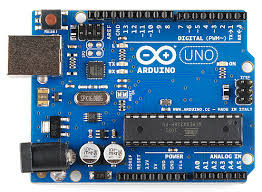
\includegraphics[width=.75\textwidth]{figures/Arduino/arduinouno.jpg}
  \caption{Ini adalah Arduino UNO}\label{fig:arduinouno}
\end{figure}
  \item Kabel Jumper seperti pada gambar \ref{fig:jumper},
  \begin{figure}[!htbp]
  \centering
  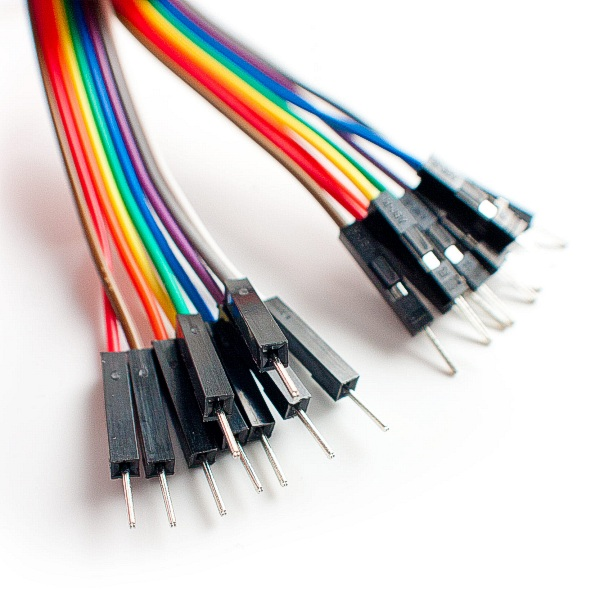
\includegraphics[width=.75\textwidth]{figures/Arduino/jumper.jpg}
  \caption{Ini adalah Kabel Jumper}\label{fig:jumper}
\end{figure}
  \item \textit{Coming Soon}
\end{enumerate}

\section{Software Pendukung}
\subsection{Simulator}
Sebelum memulai merangkai ada baiknya untuk merancang terlebih dahulu. Perancangan dilakukan agar dapat menganalisa kebutuhan baik itu perangkat keras maupun script code pendukung. Ada beberapa simulator yang dapat digunakan secara gratis misalnya VBB (Virtual Bread Board), Proteus dll. Untuk perancangan Line Follower Robotic akan menggunakan VBB.
\subsubsection{VBB (Virtual Bread Board)}


\subsection{IDE}
IDE adalah sebuah software yang berperan untuk menulis program, meng-compile menjadi kode biner dan meng-upload ke dalam memory microcontroller. Ada banyak projek dan alat-alat dikembangkan oleh akademisi dan profesional dengan menggunakan Arduino, selain itu juga ada banyak modul-modul pendukung (sensor, tampilan, penggerak dan sebagainya)yang dibuat oleh pihak lain untuk bisa disambungkan dengan Arduino. Arduino berevolusi menjadi sebuah platform karena ia menjadi pilihan dan acuan bagi banyak praktisi \cite{djuandi2011pengenalan}.

\section{Langkah-langkah} 